%!TEX program = xelatex
\documentclass[12pt, a4paper]{article}

\usepackage[dvipsnames]{xcolor}

\usepackage{fancyhdr}
\usepackage{extramarks}
\usepackage{amsmath}
\usepackage{empheq}
\usepackage{amsthm}
\usepackage{amsfonts}
\usepackage{tikz}
\usepackage[plain]{algorithm}
\usepackage{algpseudocode}

\usepackage{ctex}
\usepackage{indentfirst}
\usepackage{wrapfig}
\usetikzlibrary{automata,positioning,shapes.geometric,arrows.meta,patterns,calc}
\numberwithin{equation}{section}

%
% Basic Document Settings
%

\topmargin=-0.25in
\evensidemargin=0in
\oddsidemargin=0in
\textwidth=6.5in
\textheight=9.2in
\headsep=0.25in

\linespread{1.1}

\pagestyle{fancy}
\lhead{\hmwkAuthorName}
\chead{\hmwkClass : \hmwkTitle}
\rhead{\firstxmark}
\lfoot{\lastxmark}
\cfoot{\thepage}

\renewcommand\headrulewidth{0.4pt}
\renewcommand\footrulewidth{0.4pt}

\setlength{\parindent}{2em}  % 2em代表首行缩进两个字符

%
% Create Problem Sections
%

\newcommand{\enterProblemHeader}[1]{
    \nobreak\extramarks{}{Problem \arabic{#1} continued on next page\ldots}\nobreak{}
    \nobreak\extramarks{Problem \arabic{#1} (continued)}{Problem \arabic{#1} continued on next page\ldots}\nobreak{}
}

\newcommand{\exitProblemHeader}[1]{
    \nobreak\extramarks{Problem \arabic{#1} (continued)}{Problem \arabic{#1} continued on next page\ldots}\nobreak{}
    \stepcounter{#1}
    \nobreak\extramarks{Problem \arabic{#1}}{}\nobreak{}
}

% \setcounter{secnumdepth}{0}
\newcounter{partCounter}
\newcounter{homeworkProblemCounter}
\setcounter{homeworkProblemCounter}{0}
% \nobreak\extramarks{Problem \arabic{homeworkProblemCounter}}{}\nobreak{}

%
% Homework Problem Environment
%
% This environment takes an optional argument. When given, it will adjust the
% problem counter. This is useful for when the problems given for your
% assignment aren't sequential. See the last 3 problems of this template for an
% example.
%
\newenvironment{homeworkProblem}[1][-1]{
    \ifnum#1>0
        \setcounter{homeworkProblemCounter}{#1}
    \fi
    \section{Problem \arabic{homeworkProblemCounter}}
    \setcounter{partCounter}{1}
    \enterProblemHeader{homeworkProblemCounter}
}{
    \exitProblemHeader{homeworkProblemCounter}
}

%
% Homework Details
%   - Title
%   - Due date
%   - Class
%   - Section/Time
%   - Instructor
%   - Author
%

\newcommand{\hmwkTitle}{Vector Algebra and Spatial Geometry}
\newcommand{\hmwkDueDate}{\today}
\newcommand{\hmwkClass}{Advanced Mathematics}
\newcommand{\hmwkClassTime}{}
\newcommand{\myUniversiy}{Wuhan University}
\newcommand{\hmwkAuthorName}{\textbf{Lai Wei}}

%
% Title Page
%

\title{
    \vspace{2in}
    \textmd{\textbf{\hmwkClass:\ \hmwkTitle}}\\
    \normalsize\vspace{0.1in}\small{日期: \hmwkDueDate}\\
    \vspace{0.1in}\large{\textit{\myUniversiy}}
    \vspace{3in}
}

\author{\hmwkAuthorName}
\date{}

\renewcommand{\part}[1]{\textbf{\large Part \Alph{partCounter}}\stepcounter{partCounter}\\}

%
% Various Helper Commands
%

% Useful for algorithms
\newcommand{\alg}[1]{\textsc{\bfseries \footnotesize #1}}

% % For derivatives
% \newcommand{\deriv}[1]{\frac{\mathrm{d}}{\mathrm{d}x} (#1)}

% For partial derivatives
\newcommand{\pderiv}[2]{\frac{\partial}{\partial #1} (#2)}

% Integral dx
\newcommand{\dx}{\mathrm{d}x}

% Alias for the Solution section header
\newcommand{\solution}{\textbf{\large Solution}}

% Probability commands: Expectation, Variance, Covariance, Bias
\newcommand{\E}{\mathrm{E}}
\newcommand{\Var}{\mathrm{Var}}
\newcommand{\Cov}{\mathrm{Cov}}
\newcommand{\Bias}{\mathrm{Bias}}

% 我的newcommand
\newcommand{\degree}{^{\circ}}
\newcommand{\arrow}{-{Stealth[length=4mm,width=2mm]}}
\newcommand{\rmd}{\mathrm{d}}
\newcommand{\deriv}[2]{\frac{\rmd #1}{\rmd #2}}
\renewcommand{\parallel}{\mathrel{/\mskip-2.5mu/}}
\newcommand{\parallelogram}{
	\mathord
    {\text
        {
			\tikz[baseline]
			\draw (0,.1ex) -- (.8em,.1ex) -- (1em,1.6ex) -- (.2em,1.6ex) -- cycle;
        }
    }
}

\begin{document}

\maketitle

\pagebreak

% 设置页码格式是罗马数字
\pagenumbering{roman}

% 生成目录
\tableofcontents

\pagebreak

% 设置页码格式是阿拉伯数字
\pagenumbering{arabic}

\pagebreak

\section{向量积、混合积}

\subsection{向量积}

\subsubsection{定义}

    设有向量\(\overrightarrow{a}\)、\(\overrightarrow{b}\),其夹角为\(\theta\)。定义新向量,
    记作\(\overrightarrow{a} \times \overrightarrow{b}\),如下:

    \begin{itemize}
        \item 大小:
            \begin{align}
                \lvert \overrightarrow{a} \times \overrightarrow{b} \rvert =
                \lvert \overrightarrow{a} \rvert \cdot \lvert \overrightarrow{b} \rvert \cdot \sin\theta
            \end{align}            
        \item 方向:\(\overrightarrow{a} \times \overrightarrow{b}\)与\(\overrightarrow{a}\)、\(\overrightarrow{b}\)
            都垂直,其指向按右手螺旋定则,由\(\overrightarrow{a}\)沿着不大于\(\mathrm{\pi}\)
            的角度转向\(\overrightarrow{b}\)确定。
    \end{itemize}

\subsubsection{性质}

    \begin{enumerate}
        \item \(\overrightarrow{a} \times \overrightarrow{b} \perp \overrightarrow{a}\),
            \(\overrightarrow{a} \times \overrightarrow{b} \perp \overrightarrow{b}\)
        \item 重要结论:
        \\
        \(\overrightarrow{a} \times \overrightarrow{a} = \overrightarrow{0}\)
        \\
        对非零向量\(\overrightarrow{a}\),\(\overrightarrow{b}\),有\(\overrightarrow{a} \parallel
        \overrightarrow{b} \leftrightarrow \overrightarrow{a} \times \overrightarrow{b} = 
        \overrightarrow{0}\)
        \item 几何意义(向量积的模):
            \begin{equation}
                \begin{aligned}
                    \lvert \overrightarrow{a} \times \overrightarrow{b} \rvert &=
                    \lvert \overrightarrow{a} \rvert \cdot \lvert \overrightarrow{b} \rvert \cdot \sin\theta
                    \\
                    &= S_{\parallelogram}
                \end{aligned}        
            \end{equation}


            \[
                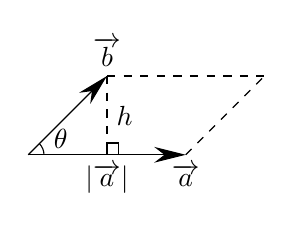
\begin{tikzpicture}
                    \coordinate[label=above:$\overrightarrow{b}$] (b) at (1,1);
                    \coordinate[label=below:$\overrightarrow{a}$] (a) at (2,0);
                    \coordinate[label=right:$\theta$] (theta) at (0.2,0.2);
                    \coordinate[label=right:$h$] (h) at (1,0.5);
                    \coordinate[label=below:$\lvert\overrightarrow{a}\rvert$] (_a_) at (1,0);
                    \draw[\arrow] (0,0) -- (a);
                    \draw[\arrow] (0,0) -- (b);
                    \draw[dashed] (b) -- (3,1);
                    \draw[dashed] (a) -- (3,1);
                    \draw (0.2,0) arc (0:45:0.2);
                    \draw[dashed] (b) -- (_a_);
                    \draw (1,0) rectangle (1.15,0.15);
                \end{tikzpicture}
            \]
            即\(\lvert \overrightarrow{a} \times \overrightarrow{b} \rvert\)表示:
            以\(\overrightarrow{a}\)、\(\overrightarrow{b}\)为邻边的平行四边形的面积。
    \end{enumerate}
    
\subsubsection{运算规律}

    \begin{enumerate}
        \item 反交换律:
            \begin{align}
                \overrightarrow{a} \times \overrightarrow{b} = 
                - \overrightarrow{b} \times \overrightarrow{a}
            \end{align}
        \item 分配律:
            \begin{align}
                \left(\overrightarrow{a} + \overrightarrow{b}\right) \times \overrightarrow{c}
                = \overrightarrow{a} \times \overrightarrow{c} + \overrightarrow{b} \times \overrightarrow{c}
            \end{align}
        \item 结合律:
            \begin{align}
                \left(\lambda \overrightarrow{a}\right) = \lambda \left(\overrightarrow{a}
                \times \overrightarrow{b}\right) = \overrightarrow{a} \times \left(\lambda \overrightarrow{b}\right)
            \end{align}
    \end{enumerate}

\subsubsection{向量积的坐标表示}

    设有向量\(\overrightarrow{a} = \left(x_1, y_1, z_1\right)\)、\(\overrightarrow{b} = \left(x_2, y_2, z_2\right)\),
    则有
    
    \begin{equation}
        \begin{aligned}
            \overrightarrow{a} \times \overrightarrow{b} &= \left(x_1\overrightarrow{i} + y_1\overrightarrow{j}
            + z_1\overrightarrow{k}\right) \times \left(x_2\overrightarrow{i} + y_2\overrightarrow{j} +
            z_2\overrightarrow{k}\right)
            \\
            &= \left(y_1z_2 - z_1y_2\right) \cdot \overrightarrow{i} + \left(z_1x_2 - x_1z_2\right) \cdot \overrightarrow{j}
            + \left(x_1y_2 - y_1x_2\right) \cdot \overrightarrow{k}
            \\
            &= \left(y_1z_2 - z_1y_2,\; z_1x_2 - x_1z_2\,\; x_1y_2 - y_1x_2\right)
            \\
            &= \left|
                \begin{array}{cccc}
                \overrightarrow{i} & \overrightarrow{j} & \overrightarrow{k} \\
                x_1 & y_1 & z_1 \\
                x_2 & y_2 & z_2
                \end{array}
            \right|
        \end{aligned}
    \end{equation}

    同理,

    \[
        \overrightarrow{b} \times \overrightarrow{a} =
        \left|
            \begin{array}{cccc}
            \overrightarrow{i} & \overrightarrow{j} & \overrightarrow{k} \\
            x_2 & y_2 & z_2 \\
            x_1 & y_1 & z_1
            \end{array}
        \right|
    \]

\subsection{混合积}

\subsubsection{定义}

    设有向量\(\overrightarrow{a}\),\(\overrightarrow{b}\),\(\overrightarrow{c}\),称数\(\left(\overrightarrow{a}
    \times \overrightarrow{b}\right) \cdot \overrightarrow{c}\)为向量\(\overrightarrow{a}\),\(\overrightarrow{b}\),
    \(\overrightarrow{c}\)的混合积,记作\(\left[\overrightarrow{a} \; \overrightarrow{b} \;
    \overrightarrow{c}\right]\),即

    \begin{align}
        \left[\overrightarrow{a} \; \overrightarrow{b} \; \overrightarrow{c}\right] =
        \left(\overrightarrow{a} \times \overrightarrow{b}\right) \cdot \overrightarrow{c}
    \end{align}

\subsubsection{坐标表示}

    设有向量\(\overrightarrow{a} = \left(x_1, y_1, z_1\right)\)、\(\overrightarrow{b} = \left(x_2, y_2, z_2\right)\)、
    \(\overrightarrow{c} = \left(x_3, y_3, z_3\right)\),则有

    \begin{align}
        \left[\overrightarrow{a} \; \overrightarrow{b} \; \overrightarrow{c}\right] =
        \left|
            \begin{array}{cccc}
            x_1 & y_1 & z_1 \\
            x_2 & y_2 & z_2 \\
            x_3 & y_3 & z_3
            \end{array}
        \right|
    \end{align}

\subsubsection{几何意义}

    \(\left|\left[\overrightarrow{a} \; \overrightarrow{b} \; \overrightarrow{c}\right]\right|\)表示以
    \(\overrightarrow{a}\),\(\overrightarrow{b}\),\(\overrightarrow{c}\)为相邻三条棱的平行六面体的体积。
    因此,\(\overrightarrow{a}\),\(\overrightarrow{b}\),\(\overrightarrow{c}\)共线\(\Leftrightarrow
    \left[\overrightarrow{a} \; \overrightarrow{b} \; \overrightarrow{c}\right] = 0\)。

\subsubsection{运算规律}

    \begin{equation}
        \begin{aligned}
            &\left[\overrightarrow{a} \; \overrightarrow{b} \; \overrightarrow{c}\right] =
            \left[\overrightarrow{b} \; \overrightarrow{c} \; \overrightarrow{a}\right] =
            \left[\overrightarrow{c} \; \overrightarrow{a} \; \overrightarrow{b}\right]
            \\
            = &- \left[\overrightarrow{a} \; \overrightarrow{c} \; \overrightarrow{b}\right] =
            - \left[\overrightarrow{c} \; \overrightarrow{b} \; \overrightarrow{a}\right] =
            - \left[\overrightarrow{b} \; \overrightarrow{a} \; \overrightarrow{c}\right]
        \end{aligned}
    \end{equation}

    即按照下图沿同一方向(顺时针或逆时针)旋转的混合积组合的值是相等的。

    \[
        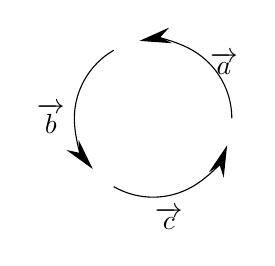
\begin{tikzpicture}
            \coordinate[label=right:$\overrightarrow{a}$] (a) at (0.6,0.7);
            \coordinate[label=left:$\overrightarrow{b}$] (b) at (-1,0);
            \coordinate[label=below:$\overrightarrow{c}$] (c) at (0.2,-1);
            \draw[\arrow] (1,0) arc (0:100:1);
            \draw[\arrow] (-0.5,1.732/2) arc (120:220:1);
            \draw[\arrow] (-0.5,-1.732/2) arc (240:340:1);
        \end{tikzpicture}
    \]

\subsubsection{例题}

    已知\((\overrightarrow{a} \times \overrightarrow{b}) \cdot \overrightarrow{c} = 2\),求\(\left[(\overrightarrow{a} \times \overrightarrow{b}) \times
    (\overrightarrow{b} + \overrightarrow{c})\right] \cdot (\overrightarrow{c} + \overrightarrow{a})\)。

    \textbf{Solution}
    \\


    \[
        \begin{split}
            & \left[(\overrightarrow{a} \times \overrightarrow{b}) \times (\overrightarrow{b} + \overrightarrow{c})\right] \cdot (\overrightarrow{c} + \overrightarrow{a})
            \\
            &= \left[\overrightarrow{a} \times \overrightarrow{b} + \overrightarrow{a} \times \overrightarrow{c} + \overrightarrow{b} \times \overrightarrow{b} +
            \overrightarrow{b} \times \overrightarrow{c}\right] \cdot (\overrightarrow{c} + \overrightarrow{a})
        \end{split}
    \]

    由\(\overrightarrow{b} \times \overrightarrow{b} = 0\),故
    \\

    \[
        \begin{split}
            & \left[(\overrightarrow{a} \times \overrightarrow{b}) \times (\overrightarrow{b} + \overrightarrow{c})\right] \cdot (\overrightarrow{c} + \overrightarrow{a})
            \\
            &= \left[\overrightarrow{a} \times \overrightarrow{b} + \overrightarrow{a} \times \overrightarrow{c} + \overrightarrow{b} \times \overrightarrow{c}\right]
            \cdot (\overrightarrow{c} + \overrightarrow{a})
            \\
            &= \left[\overrightarrow{a} \; \overrightarrow{b} \; \overrightarrow{c}\right] + \left[\overrightarrow{a} \; \overrightarrow{c} \; \overrightarrow{c}\right] + 
            \left[\overrightarrow{b} \; \overrightarrow{c} \; \overrightarrow{c}\right] + \left[\overrightarrow{a} \; \overrightarrow{b} \; \overrightarrow{a}\right] +
            \left[\overrightarrow{a} \; \overrightarrow{c} \; \overrightarrow{a}\right] + \left[\overrightarrow{b} \; \overrightarrow{c} \; \overrightarrow{a}\right]
        \end{split}
    \]

    显然,当混合积中只有不同的两个向量时(可认为这三个向量共面),该混合积值为0。于是

    \[
        \begin{split}
            & \left[(\overrightarrow{a} \times \overrightarrow{b}) \times (\overrightarrow{b} + \overrightarrow{c})\right] \times (\overrightarrow{c} + \overrightarrow{a})
            \\
            &= \left[\overrightarrow{a} \; \overrightarrow{b} \; \overrightarrow{c}\right] + \left[\overrightarrow{b} \; \overrightarrow{c} \; \overrightarrow{a}\right]
        \end{split}
    \]

    由于

    \[
        \left[\overrightarrow{a} \; \overrightarrow{b} \; \overrightarrow{c}\right] =
        \begin{vmatrix}
        a_{x} & a_{y} & a_{z} \\
        b_{x} & b_{y} & b_{z} \\
        c_{x} & c_{y} & c_{z}
        \end{vmatrix}
    \]

    而

    \[
        \left[\overrightarrow{b} \; \overrightarrow{c} \; \overrightarrow{a}\right] =
        \begin{vmatrix}
        b_{x} & b_{y} & b_{z} \\
        c_{x} & c_{y} & c_{z} \\
        a_{x} & a_{y} & a_{z}
        \end{vmatrix}
    \]

    所以

    \[
    \left[\overrightarrow{a} \; \overrightarrow{b} \; \overrightarrow{c}\right] = \left[\overrightarrow{b} \; \overrightarrow{c} \; \overrightarrow{a}\right]
    \]

    于是

    \[
        \begin{split}
            \left[(\overrightarrow{a} \times \overrightarrow{b}) \times (\overrightarrow{b} + \overrightarrow{c})\right] \times (\overrightarrow{c} + \overrightarrow{a})
            = 2 \; \left[\overrightarrow{a} \; \overrightarrow{b} \; \overrightarrow{c}\right]
        \end{split}
    \]

\section{平面及其方程}

\subsection{曲面方程与空间曲线方程的概念}

\subsubsection{曲面方程}

    设有曲面\(S: F\left(x, y, z\right) = 0\),满足

    \begin{enumerate}
        \item 曲面\(S\)上任一点都满足方程;
        \item 不在曲面\(S\)上的点的坐标不满足方程。
    \end{enumerate}

\subsubsection{空间曲线方程}

    设有曲面\(S_1: F_1\left(x, y, z\right) = 0\)和设有曲面\(S_2: F_2\left(x, y, z\right) = 0\),
    联立两方程:

    \[
        \begin{cases}
            F_1\left(x, y, z\right) = 0, \\
            F_2\left(x, y, z\right) = 0.
        \end{cases}
    \]

    满足

    \begin{enumerate}
        \item 曲面\(S\)上任一点都满足方程;
        \item 不在曲面\(S\)上的点的坐标不满足方程。
    \end{enumerate}

\subsection{平面的点法式方程}

    设平面\(\mathit{\Pi}\)上有一点\(M_{0}\left(x_0,y_0,z_0\right)\),其法向量为\(\overrightarrow{n} = \left(
    A, B, C\right)\)。(注意:平面的法向量不唯一。)
    
    设\(M\left(x,y,z\right)\),则\(\overrightarrow{M_{0}M} \perp \overrightarrow{n}\),则
    \(\overrightarrow{M_{0}M} \cdot \overrightarrow{n} = 0\),而\(\overrightarrow{M_{0}M} =
    \left(x-x_0,y-y_0,z-z_0\right)\)。于是
    
    \begin{align}
        A\left(x-x_0\right) + B\left(y-y_0\right) + C\left(z-z_0\right) = 0
        \label{Point-Normal-Plane}
    \end{align}
    
    即为平面\(\mathit{\Pi}\)的点法式方程。

\subsection{平面的一般方程}

    \begin{align}
        Ax + By + Cz + D = 0
        \label{General-Form-Plane}
    \end{align}

    即为平面的一般方程。

    任一三元一次方程的图形总是一个平面,方程\ref{General-Form-Plane}中\(x\)、\(y\)、\(z\)的系数就是该平面的
    一个法向量\(\overrightarrow{n}\)的坐标,即\(\overrightarrow{n} = \left(A, B, C\right)\)。

    特殊情况:

    \begin{enumerate}
        \item \(D=0 \Leftrightarrow \)平面通过原点;
        \item \(A=0 \Leftrightarrow \)平面平行于(或包含)\(x\)轴;
            \\
            \(B=0 \Leftrightarrow \)平面平行于(或包含)\(y\)轴;
            \\
            \(C=0 \Leftrightarrow \)平面平行于(或包含)\(z\)轴;
        \item \(A=B=0 \Leftrightarrow \)平面平行于(或重合于)\(xOy\)平面;
            \\
            \(B=C=0 \Leftrightarrow \)平面平行于(或重合于)\(yOz\)平面;
            \\
            \(A=C=0 \Leftrightarrow \)平面平行于(或重合于)\(xOz\)平面;
        \item \(A=D=0 \Leftrightarrow \)平面包含\(x\)轴;
            \\
            \(B=D=0 \Leftrightarrow \)平面包含\(y\)轴;
            \\
            \(C=D=0 \Leftrightarrow \)平面包含\(z\)轴;
        \item \(A=B=D=0 \Leftrightarrow z=0\)(\(xOy\)平面);
            \\
            \(B=C=D=0 \Leftrightarrow x=0\)(\(yOz\)平面);
            \\
            \(A=C=D=0 \Leftrightarrow y=0\)(\(xOz\)平面);
    \end{enumerate}

\subsection{平面的截距式方程}

    \begin{align}
        \frac{x}{a} + \frac{y}{b} + \frac{z}{c} = 1
        \label{Intercept-Form-Plane}
    \end{align}

    即为平面的截距式方程。方程\ref{Intercept-Form-Plane}中\(a\),\(b\),\(c\)即分别为平面在\(x\),\(y\),\(z\)
    轴上的截距。

\subsection{两平面的夹角}

\subsubsection{定义}

    两平面的法线向量的夹角(通常指锐角或直角)称为两平面的夹角。因此\(\cos \theta = \left|\cos
    \left(\hat{\overrightarrow{n_1}, \overrightarrow{n_2}}\right)\right|\)。

    设平面\(\mathit{\Pi_{1}}\)和\(\mathit{\Pi_{2}}\)的法线向量依次为\(\overrightarrow{n_{1}} = \left(A_{1}, B_{1}, C_{1}\right)\),
    \(\overrightarrow{n_{2}} = \left(A_{2}, B_{2}, C_{2}\right)\)。按两向量夹角的余弦的坐标表示式平面\(\mathit{\Pi_{1}}\)
    和\(\mathit{\Pi_{2}}\)的夹角\(\theta\)可由

    \begin{align}
        \cos \theta=\frac{\left|A_1 A_2+B_1 B_2+C_1 C_2\right|}
        {\sqrt{A_1^2+B_1^2+C_1^2} \sqrt{A_2^2+B_2^2+C_2^2}}
    \end{align}

    来确定。

\subsubsection{结论}

    \begin{enumerate}
        \item \(\mathit{\Pi_{1}}\)和\(\mathit{\Pi_{2}}\)相互垂直相当于\(A_1 A_2+B_1 B_2+C_1 C_2=0\)
        \item \(\mathit{\Pi_{1}}\)和\(\mathit{\Pi_{2}}\)相互平行相当于\(\dfrac{A_1}{A_2}=\dfrac{B_1}{B_2}=\dfrac{C_1}{C_2}\)
    \end{enumerate}

\subsection{点到平面的距离}

    设点\(P_{0}\left(x_0, y_0, z_0\right)\)是平面\(Ax + By + Cz + D = 0\)外一点,则\(P_0\)到该平面的距离为

    \begin{align}
        d=\frac{\left|A x_0+B y_0+C z_0\right|}{\sqrt{A^2+B^2+C^2}}
    \end{align}

    设有两平行平面\(\mathit{\Pi_{1}}: Ax + By +Cz +D_1 = 0\)和\(\mathit{\Pi_{1}}: Ax + By +Cz +D_2 = 0\),则两平面间的距离为

    \begin{align}
        d=\frac{\left|D_1 - D_2\right|}{\sqrt{A^2+B^2+C^2}}
    \end{align}

\section{空间直线及其方程}

\subsection{空间直线的一般方程}

    \begin{equation}
        L:\left\{\begin{array}{l}
        A_1 x+B_1 y+C_1 z+D_1=0 \\
        A_2 x+B_2 y+C_2 z=D_2=0
        \end{array}\right.
    \end{equation}

    注意:空间直线的方程是不唯一的。

\subsection{空间直线的对称式方程}

    \(L\)上有一点\(M_0\left(x_0, y_0, z_0\right)\),非零方向向量\(\overrightarrow{s} =
    \left(m, n, p\right)\),设\(L\)上任一点\(M_0\left(x, y, z\right)\),则
    \(\overrightarrow{M_{0}M} \parallel \overrightarrow{s}\),而\(\overrightarrow{M_{0}M} =
    \left(x-x_0, y-y_0, z-z_0\right)\),所以

    \begin{align}
        \frac{x-x_0}{m}=\frac{y-y}{n}=\frac{z-z_0}{p}
    \end{align}

    即为直线的对称式方程(或称点向式方程)
    
    注意

    \begin{enumerate}
        \item 非零向量\(\overrightarrow{s} = \left(m, n, p\right)\)称为\(L\)的方向向量(不唯一);
        \item 直线上任一方向向量\(\overrightarrow{s}\)的坐标\(m, n, p\)称为一组方向数;
        \item \(\overrightarrow{s}\)的方向余弦叫做\(L\)的方向余弦;
        \item 当\(m = 0\)时,
            \begin{align}
                \left\{\begin{array}{l}
                x-x_0=0 \\
                \dfrac{y-y_0}{n}=\dfrac{z-z_0}{p}
                \end{array}\right.
            \end{align}
        \item 当\(m = n = 0\)时,
            \begin{equation}
                \left\{\begin{array}{l}
                x-x_0=0 \\
                y-y_0=0
                \end{array}\right.
            \end{equation}

            此时,直线与\(z\)轴平行。
    \end{enumerate}

\subsection{空间直线的参数方程}

    令$\dfrac{x-x_0}{m}=\dfrac{y-y_0}{n}=\dfrac{z-z_0}{p}=t$,则

    \begin{equation}
        \left\{\begin{array}{l}
        x=x_0+m t \\
        y=y_0+n t \\
        z=z_0+p t
        \end{array}\right.
    \end{equation}

    注意:

    \begin{enumerate}
        \item \(t\)取定每一个值,对应\(x, y, z\)为\(L\)上一点的坐标;
        \item 参数式方程一般用来求直线与平面的交点。
    \end{enumerate}

\subsection{空间直线的两点式方程}

    过\(M_1\left(x_1, y_1, z_1\right)\)和\(M_2\left(x_2, y_2, z_2\right)\)两点的直线方程,
    则方向向量\(\overrightarrow{s} = \overrightarrow{M_{1}M_{2}} = \\
    \left(x_2-x_1, y_2-y_1, z_2-z_1\right)\)。

    所以方程为

    \begin{equation}
        \frac{x-x_1}{x_2-x_1}=\frac{y-y_1}{y_2-y_1}=\frac{z-z_1}{z_2-z_1}
    \end{equation}

    即为直线的两点式方程。

\subsection{两直线的夹角}

\subsubsection{定义}

    两直线的方向向量的夹角(通常指锐角或直角)。

\subsubsection{夹角的余弦公式}

    设直线的方向向量为\(\overrightarrow{s} = \left(m, n, p\right)\),平面的法线向量为
    \(\overrightarrow{n} = \left(A, B, C\right)\),则直线和平面的夹角\(\varphi\)
    可由

    \begin{equation}
        \cos \varphi=\frac{\left|m_1 m_2+n_1 n_2+p_1 p_2\right|}{\sqrt{m_1^2+n_1^2+p_1^2} \sqrt{m_2^2+n_2^2+p_2^2}}
    \end{equation}

    来确定。

    于是可知:

    \begin{enumerate}
        \item \(L_1 \perp L_2 \Leftrightarrow \overrightarrow{s_1} \perp \overrightarrow{s_2}
            \Leftrightarrow \overrightarrow{s_1} \cdot \overrightarrow{s_2} \Leftrightarrow
            m_1 m_2+n_1 n_2+p_1 p_2 = 0\)
        \item \(L_1 \parallel L_2 \Leftrightarrow \overrightarrow{s_1} \parallel \overrightarrow{s_2}
        \Leftrightarrow \dfrac{m_1}{m_2}=\dfrac{n_1}{n_2}=\dfrac{p_1}{p_2}\)
    \end{enumerate}

\subsection{直线与平面的夹角}

\subsubsection{定义}

    直线\(L\)与其在平面上投影直线所形成的夹角。

\subsubsection{夹角的正弦公式}

    设直线\(L_1\)和\(L_2\)的方向向量依次为\(\overrightarrow{s_1} = \left(m_1, n_1, p_1\right)\)和
    \(\overrightarrow{s_2} = \left(m_2, n_2, p_2\right)\),则直线\(L_1\)和\(L_2\)的夹角\(\varphi\)
    可由

    \begin{equation}
        \sin \varphi=\frac{|A m+B n+C p|}{\sqrt{A^2+B^2+C^2} \sqrt{m^2+n^2+p^2}}
    \end{equation}

    来确定。

    于是可知

    \begin{enumerate}
        \item $ L \parallel \mathit{\Pi} \Leftrightarrow \overrightarrow{s} \perp \overrightarrow{x} \Leftrightarrow
            \overrightarrow{s} \cdot \overrightarrow{n}=0 \Leftrightarrow Amn+Bn+Cp=0$
        \item $L \perp \mathit{\Pi} \Leftrightarrow \overrightarrow{s} \parallel \overrightarrow{x} \Leftrightarrow
            \dfrac{A}{m}=\dfrac{B}{n}=\dfrac{c}{p}$.
    \end{enumerate}

\subsection{平面束方程}

    设直线\(L\)由方程

    \begin{empheq}[left=\empheqlbrace]{align}
        A_1 x + B_1 y + C_1 z + D_1 &= 0 \\
        A_2 x + B_2 y + C_2 z + D_2 &= 0 \label{Pencil-Planes-2}
    \end{empheq}

    给出,其中\(A_1, B_1, C_1\)与\(A_2, B_2, C_2\)不成比例,则

    \begin{equation}
        A_1 x+B_1 y+C_1 z+D_1+\lambda\left(A_2x+B_2y+C_2z+D_2\right) = 0
    \end{equation}

    能表示通过直线\(L\)的所有平面(除平面\ref{Pencil-Planes-2}外)。则称之为直线\(L\)的平面束方程。

\subsection{例题}

\subsubsection{Problem 1}

    将一般方程$L:\left\{\begin{array}{l}x+y+z+1=0 \\ 2 x-y+3z+4=0\end{array}\right.$
    化为对称式、参数式并求\(L\)与平面\(\mathit{\Pi}: x + y =0\)的交点。
    \\

    \textbf{Solution}
    \\

    取\(y = 0\),代入方程中,得\(x=1,\; z=-2\),则点\(M_{0}\left(1,0,-2\right)\)为\(L\)上一点;
    取\(z = 0\),代入方程中,得\(x=-\frac{5}{3},\; y=\frac{2}{3}\),
    则点\(M_{0}\left(-\frac{5}{3},\frac{2}{3},0\right)\)为\(L\)上一点。

    则\(\overrightarrow{M_{0}M_{1}} = \left(-\frac{8}{3},\frac{2}{3},2\right)\),
    取\(\overrightarrow{s} = \left(4,1,3\right)\),则\(L\)的对称式方程为

    \[
        \frac{x-1}{-4}=\frac{y-0}{1}=\frac{z+2}{3}
    \]

    则\(L\)的参数式方程为

    $$
        \left\{\begin{array}{l}
        x=-4 t \\
        y=t \\
        z=-2+3 t
        \end{array}\right.
    $$

    将参数式方程代入平面\(\mathit{\Pi}: x + y =0\)中,则有\(\left(1-4t\right) + t = 0\),所以
    \(t = \frac{1}{3}\)。

    所以\(L\)与平面\(\mathit{\Pi}: x + y =0\)的交点为\(\left(-\frac{1}{3},\frac{1}{3},-1\right)\)。

\subsubsection{Problem 2}

    求过点\(\left(2,1,3\right)\)且与直线$\dfrac{x+1}{3}=\dfrac{y-1}{2}=\dfrac{z}{-1}$垂直相交的
    直线的方程。
    \\

    \textbf{Solution}
    \\

    \textbf{Part One}

    \begin{wrapfigure}{r}{4cm}
        \centering
        \includegraphics[scale=0.08]{"Chapter 08 images/pic1.png"}
        % \caption{}
        \label{pic1}
    \end{wrapfigure}

    要求过点\(M_{0}\left(2,1,3\right)\)且与直线$L$垂直相交的直线,关键在于求垂足\(M_1\)。
    可以作过点\(M_{0}\)且垂直于直线$L$的平面。

    则该平面的对称式方程为

    \[
        3(x-2)+2(y-1)-(z-3)=0
    \]

    即

    \[
        3x + 2y -z -5 =0
    \]

    \textbf{Part Two}

    再求直线与垂直平面的交点:

    令$\dfrac{x+1}{3}=\dfrac{y-1}{2}=\dfrac{z}{1}=t$

    得

    $$
        \left\{\begin{array}{l}
        x=-1+3 t \\
        y=1+2 t \\
        z=-t
        \end{array}\right.
    $$

    解得\(t=\dfrac{3}{7}\)

    代入得交点坐标为$\left(\dfrac{2}{7}, \dfrac{13}{7},-\dfrac{3}{7}\right)$

    \textbf{Part Three}

    所以所求直线的一个方向向量为

    $$
        \left(\frac{2}{7}-2, \frac{13}{7}-1,-\frac{3}{7}-3\right)=-\frac{6}{7}(2,-1,4)
    $$

    所以所求的直线方程为

    $$
        \frac{x-2}{2}=\frac{y-1}{-1}=\frac{z-3}{4}
    $$

\subsubsection{Problem 3}

    求直线$\left\{\begin{array}{l}x+y-z-1=0 \\ x-y+z+1=0\end{array}\right.$在平面\(x+y+z=0\)上投影
    直线的方程。
    \\

    \textbf{Solution}
    \\

    \begin{wrapfigure}{r}{4cm}
        \centering
        \includegraphics[scale=0.08]{"Chapter 08 images/pic2.png"}
        % \caption{}
        \label{pic2}
    \end{wrapfigure}

    过直线$\left\{\begin{array}{l}x+y-z-1=0 \\ x-y+z+1=0\end{array}\right.$的平面束方程为

    $$
        (x+y-z-1)+\lambda(x-y+z+1)=0
    $$

    整理得

    $$
        (1+\lambda) x+(1-\lambda) y+(-1+\lambda) z+(-1+\lambda)=0
    $$

    由于此平面与平面\(x+y+z=0\)垂直,则两平面法向量也相互垂直。即

    $$
        (1+\lambda) \cdot 1+(1-\lambda) \cdot 1+(-1+\lambda) \cdot 1=0
    $$

    解得\(\lambda=-1\)。

    代入平面束方程中,知投影直线的方程为

    $$
        \left\{\begin{array}{l}
        y-z-1=0 \\
        x+y+z=0
        \end{array}\right.
    $$


\end{document}
